\chapter{Cuda Overview}\label{sec:i}
Cuda is a software layer that allow programmers to exploit the capability of Nvidia GPUs as general purpose processors.\\
Dealing with a video card in this way requires approaching a completely new programming style and acquiring some knowledge about the basic Nvidia GPUs architectures, even though all the internal details are masked by the framework.\\
%First of all, as a philosophical remark, a GPU cannot run anything conceived and written for a CPU, as every vector stream architecture. In order to product software that can be executed on a Cuda Capable GPU, the programmer must write natively parallel code using one of the supported languages, extended with ad hoc Cuda primitives. There is no tool that can perform automatic porting of a sequential code into a parallel one.\\
Cuda exposes the GPU as a "Parallel Co-Processor" that can be used by the CPU to speed-up the computations. More in detail, the CPU - Host - can take advantage of the high amount of parallel threads executable by the GPU - Device - to accellerate parts of a program that are specially well suitted to exploit TLP. According to this, the CPU must directly manage the program execution settings on the GPU, provide the data for the computation to the device and collect the outputs when it has done.\\
One of the most important feature of Cuda is that it abstracts away all the physical details of the supported GPUs and shows to the programmer always the very same logical organization (Figure 3.1). These GPUs can be considered a MIMD array of SIMD processors, called MultiProcessors. Each MultiProcessor is mainly composed by 3 logic elements: a fixed number of cores, an instruction unit and a private memory space. All the MultiProcessors share a pubblic memory space referred to as Device Memory in order to distinguish it from the CPU memory space - Host Memory - that is not directly accessed by the GPU. Due to the property of abstraction mentioned before, the only difference between families of Nvidia products is in the amount of memory, the number of MultiProcessor and the nature of the cores.\\

\begin{figure}[h!bt]
	\centerline{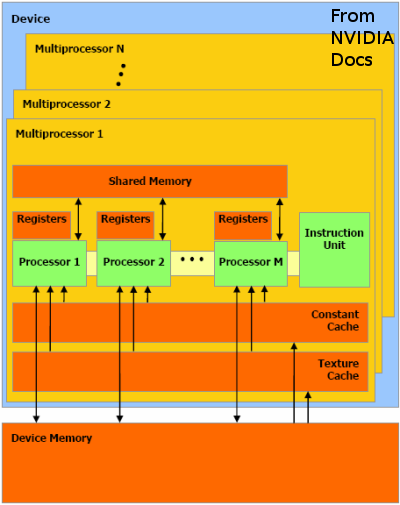
\includegraphics[width=0.5\textwidth]{img/HWModel.png}}
	\caption{Logical Organization of all the Cuda capable devices. The programmer does not have to take care of the physical organization of the GPU that will actually execute the program.}
	\label{fig:NvidiaGPUsLogicalOrg}
\end{figure}

\section{Multiprocessors}
Even if the architectural details on the Cuda capable GPU can significantly differ from a product to another, some common guidelines can be identified. The computational units of these GPUs are designed to be as simple and fast as possible. In order to keep low the complexity of the MPs, there are no branch predictors, nor any mechanisms to rollback incorrect results. Even if this can seems a serious limitation to the performance, it allow the cores of the MP to be completely focused on the arithmetic intensity. As results of this choice, the MP of the most recent Nvidia products are able to perform a double precision MAD (or MUL or ADD) per clock cycle.\\

\section{Memory Hierarchy}
The Cuda memory hierarchy consists of several elements optimized for different memory usages.\\
The Device Memory is the main memory space of the Video Card. It can be accessed by both the CPU and the GPU using different policies, usually with a latency of some hundred of clock cycles. In order to avoid confusion, it is logically partitioned into three logic component, depending on the access method: the Global Memory, that follow the common 32-,64-, or 128-byte memory transactions paradigm; Texture Memory, accessed by texture fetching; Constant Memory, managed by special operations.\\
The Global Memory is the most frequently employed memory space. Usually it is used by the CPU to load the data for the computations into the device and by the GPU to provide the results. Furthermore the Global Memory is the only space completely shared among all the SPs of the defice, for this reason it is also exploited for comunication among SPs belonging to different MPs. The Texture Memory can be written by the CPU using the Cuda API and readed by the GPU via texture fetching. No GPU texture write mechanism is provided. The Constant memory is a small special memory space that can be used for allocation of variables frequently readed. These variables must be allocated by the CPU before the execution on GPU, that can access them only in read-mode.\\ 
Due to the high latency of the Device Memory, each MP is provided of a private low latency memory space, logically composed by: a so called Shared Memory, directly accessible by all the SPs of the MP; a Constant Cache and a Texture Cache, managed by the framework; a set of exclusive Registers for each SP.\\
The Shared Memory can be considered as both a sort of cache of the Global Memory directly administrated by the cores in the MP and a mechanism for comunications among SPs belonging to the same MP. The Constant Cache and the Texture Cache are L1 caches used to speed-up the access time of the Constant Memory and the Texture Memory respectively. Due to the fact that Constant Memory and Texture Memory are read-only from the point of view of the GPU, no cache coherency protocol is needed.\\ 

\section{Programming Model}
As stated at the beginning of this chapter, the Cuda framework enable the programmer to take advantage of the high number of parallel threads executable by the GPU to expoit TLP: ideally the program is organized into identical sub-problems - working on different data - that can be solved independently. Each of this sub-problems, called Kernel, is mapped into a thread that will be executed on a SP.\\
All the threads executed by the SPs of a single MP are logically organized into a structure called Block. Virtually all the Threads belonging to a Block are execuded in parallel. Actually the number of SPs in a MP is usually much less than the number of Threads in a Block, for this reason only a part of the Threads is in concurrent execution at a given time, the so called Warp. When a MP is charged of a Block, it partitions this into warp that get sheduled by a warp sheduler for the execution on that MP. Due to the fact that all the Threads of a Block are executed on the same MP, it should be noticed that they share all the MP resources (i.e. Shared Memory and Caches) and that they can be synchronized using a specific API barrier.\\
All the Blocks are groupped into another logical structure called Grid. Considering that the number of Blocks of the Grid is usually greater than the numper of MPs, not all the Blocks can be sheduled at the same time. Since the blocks are unordered, they can execute equally well on a GPU that can handle one block at a time and one that executes a dozen or a hundred at a time, as demonstration of the scalability offered by the framework. In order to avoid complicating the Block scheduling process, no extra-block threads syncronization mechanism is provided.\\ 

\begin{figure}[h!bt]
	\centerline{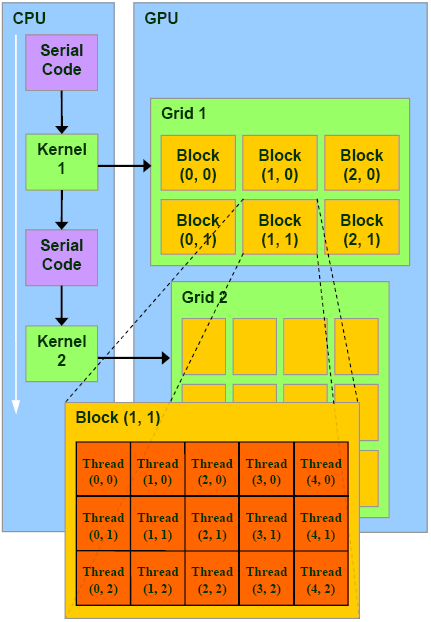
\includegraphics[width=0.5\textwidth]{img/NvidiaExecutionModel.png}}
	\caption{Nvidia Execution Model, an example of eterogeneous programming.}
	\label{fig:NvidiaGPUsLogicalOrg}
\end{figure}

\section{Best Pratices}

